% Options for packages loaded elsewhere
\PassOptionsToPackage{unicode}{hyperref}
\PassOptionsToPackage{hyphens}{url}
\PassOptionsToPackage{dvipsnames,svgnames,x11names}{xcolor}
%
\documentclass[
  letterpaper,
  DIV=11,
  numbers=noendperiod,
  oneside]{scrreprt}

\usepackage{amsmath,amssymb}
\usepackage{lmodern}
\usepackage{iftex}
\ifPDFTeX
  \usepackage[T1]{fontenc}
  \usepackage[utf8]{inputenc}
  \usepackage{textcomp} % provide euro and other symbols
\else % if luatex or xetex
  \usepackage{unicode-math}
  \defaultfontfeatures{Scale=MatchLowercase}
  \defaultfontfeatures[\rmfamily]{Ligatures=TeX,Scale=1}
\fi
% Use upquote if available, for straight quotes in verbatim environments
\IfFileExists{upquote.sty}{\usepackage{upquote}}{}
\IfFileExists{microtype.sty}{% use microtype if available
  \usepackage[]{microtype}
  \UseMicrotypeSet[protrusion]{basicmath} % disable protrusion for tt fonts
}{}
\makeatletter
\@ifundefined{KOMAClassName}{% if non-KOMA class
  \IfFileExists{parskip.sty}{%
    \usepackage{parskip}
  }{% else
    \setlength{\parindent}{0pt}
    \setlength{\parskip}{6pt plus 2pt minus 1pt}}
}{% if KOMA class
  \KOMAoptions{parskip=half}}
\makeatother
\usepackage{xcolor}
\usepackage[left=1in,marginparwidth=2.0666666666667in,textwidth=4.1333333333333in,marginparsep=0.3in]{geometry}
\setlength{\emergencystretch}{3em} % prevent overfull lines
\setcounter{secnumdepth}{5}
% Make \paragraph and \subparagraph free-standing
\ifx\paragraph\undefined\else
  \let\oldparagraph\paragraph
  \renewcommand{\paragraph}[1]{\oldparagraph{#1}\mbox{}}
\fi
\ifx\subparagraph\undefined\else
  \let\oldsubparagraph\subparagraph
  \renewcommand{\subparagraph}[1]{\oldsubparagraph{#1}\mbox{}}
\fi

\usepackage{color}
\usepackage{fancyvrb}
\newcommand{\VerbBar}{|}
\newcommand{\VERB}{\Verb[commandchars=\\\{\}]}
\DefineVerbatimEnvironment{Highlighting}{Verbatim}{commandchars=\\\{\}}
% Add ',fontsize=\small' for more characters per line
\usepackage{framed}
\definecolor{shadecolor}{RGB}{241,243,245}
\newenvironment{Shaded}{\begin{snugshade}}{\end{snugshade}}
\newcommand{\AlertTok}[1]{\textcolor[rgb]{0.68,0.00,0.00}{#1}}
\newcommand{\AnnotationTok}[1]{\textcolor[rgb]{0.37,0.37,0.37}{#1}}
\newcommand{\AttributeTok}[1]{\textcolor[rgb]{0.40,0.45,0.13}{#1}}
\newcommand{\BaseNTok}[1]{\textcolor[rgb]{0.68,0.00,0.00}{#1}}
\newcommand{\BuiltInTok}[1]{\textcolor[rgb]{0.00,0.23,0.31}{#1}}
\newcommand{\CharTok}[1]{\textcolor[rgb]{0.13,0.47,0.30}{#1}}
\newcommand{\CommentTok}[1]{\textcolor[rgb]{0.37,0.37,0.37}{#1}}
\newcommand{\CommentVarTok}[1]{\textcolor[rgb]{0.37,0.37,0.37}{\textit{#1}}}
\newcommand{\ConstantTok}[1]{\textcolor[rgb]{0.56,0.35,0.01}{#1}}
\newcommand{\ControlFlowTok}[1]{\textcolor[rgb]{0.00,0.23,0.31}{#1}}
\newcommand{\DataTypeTok}[1]{\textcolor[rgb]{0.68,0.00,0.00}{#1}}
\newcommand{\DecValTok}[1]{\textcolor[rgb]{0.68,0.00,0.00}{#1}}
\newcommand{\DocumentationTok}[1]{\textcolor[rgb]{0.37,0.37,0.37}{\textit{#1}}}
\newcommand{\ErrorTok}[1]{\textcolor[rgb]{0.68,0.00,0.00}{#1}}
\newcommand{\ExtensionTok}[1]{\textcolor[rgb]{0.00,0.23,0.31}{#1}}
\newcommand{\FloatTok}[1]{\textcolor[rgb]{0.68,0.00,0.00}{#1}}
\newcommand{\FunctionTok}[1]{\textcolor[rgb]{0.28,0.35,0.67}{#1}}
\newcommand{\ImportTok}[1]{\textcolor[rgb]{0.00,0.46,0.62}{#1}}
\newcommand{\InformationTok}[1]{\textcolor[rgb]{0.37,0.37,0.37}{#1}}
\newcommand{\KeywordTok}[1]{\textcolor[rgb]{0.00,0.23,0.31}{#1}}
\newcommand{\NormalTok}[1]{\textcolor[rgb]{0.00,0.23,0.31}{#1}}
\newcommand{\OperatorTok}[1]{\textcolor[rgb]{0.37,0.37,0.37}{#1}}
\newcommand{\OtherTok}[1]{\textcolor[rgb]{0.00,0.23,0.31}{#1}}
\newcommand{\PreprocessorTok}[1]{\textcolor[rgb]{0.68,0.00,0.00}{#1}}
\newcommand{\RegionMarkerTok}[1]{\textcolor[rgb]{0.00,0.23,0.31}{#1}}
\newcommand{\SpecialCharTok}[1]{\textcolor[rgb]{0.37,0.37,0.37}{#1}}
\newcommand{\SpecialStringTok}[1]{\textcolor[rgb]{0.13,0.47,0.30}{#1}}
\newcommand{\StringTok}[1]{\textcolor[rgb]{0.13,0.47,0.30}{#1}}
\newcommand{\VariableTok}[1]{\textcolor[rgb]{0.07,0.07,0.07}{#1}}
\newcommand{\VerbatimStringTok}[1]{\textcolor[rgb]{0.13,0.47,0.30}{#1}}
\newcommand{\WarningTok}[1]{\textcolor[rgb]{0.37,0.37,0.37}{\textit{#1}}}

\providecommand{\tightlist}{%
  \setlength{\itemsep}{0pt}\setlength{\parskip}{0pt}}\usepackage{longtable,booktabs,array}
\usepackage{calc} % for calculating minipage widths
% Correct order of tables after \paragraph or \subparagraph
\usepackage{etoolbox}
\makeatletter
\patchcmd\longtable{\par}{\if@noskipsec\mbox{}\fi\par}{}{}
\makeatother
% Allow footnotes in longtable head/foot
\IfFileExists{footnotehyper.sty}{\usepackage{footnotehyper}}{\usepackage{footnote}}
\makesavenoteenv{longtable}
\usepackage{graphicx}
\makeatletter
\def\maxwidth{\ifdim\Gin@nat@width>\linewidth\linewidth\else\Gin@nat@width\fi}
\def\maxheight{\ifdim\Gin@nat@height>\textheight\textheight\else\Gin@nat@height\fi}
\makeatother
% Scale images if necessary, so that they will not overflow the page
% margins by default, and it is still possible to overwrite the defaults
% using explicit options in \includegraphics[width, height, ...]{}
\setkeys{Gin}{width=\maxwidth,height=\maxheight,keepaspectratio}
% Set default figure placement to htbp
\makeatletter
\def\fps@figure{htbp}
\makeatother
\newlength{\cslhangindent}
\setlength{\cslhangindent}{1.5em}
\newlength{\csllabelwidth}
\setlength{\csllabelwidth}{3em}
\newlength{\cslentryspacingunit} % times entry-spacing
\setlength{\cslentryspacingunit}{\parskip}
\newenvironment{CSLReferences}[2] % #1 hanging-ident, #2 entry spacing
 {% don't indent paragraphs
  \setlength{\parindent}{0pt}
  % turn on hanging indent if param 1 is 1
  \ifodd #1
  \let\oldpar\par
  \def\par{\hangindent=\cslhangindent\oldpar}
  \fi
  % set entry spacing
  \setlength{\parskip}{#2\cslentryspacingunit}
 }%
 {}
\usepackage{calc}
\newcommand{\CSLBlock}[1]{#1\hfill\break}
\newcommand{\CSLLeftMargin}[1]{\parbox[t]{\csllabelwidth}{#1}}
\newcommand{\CSLRightInline}[1]{\parbox[t]{\linewidth - \csllabelwidth}{#1}\break}
\newcommand{\CSLIndent}[1]{\hspace{\cslhangindent}#1}

\KOMAoption{captions}{tableheading}
\makeatletter
\@ifpackageloaded{tcolorbox}{}{\usepackage[many]{tcolorbox}}
\@ifpackageloaded{fontawesome5}{}{\usepackage{fontawesome5}}
\definecolor{quarto-callout-color}{HTML}{909090}
\definecolor{quarto-callout-note-color}{HTML}{0758E5}
\definecolor{quarto-callout-important-color}{HTML}{CC1914}
\definecolor{quarto-callout-warning-color}{HTML}{EB9113}
\definecolor{quarto-callout-tip-color}{HTML}{00A047}
\definecolor{quarto-callout-caution-color}{HTML}{FC5300}
\definecolor{quarto-callout-color-frame}{HTML}{acacac}
\definecolor{quarto-callout-note-color-frame}{HTML}{4582ec}
\definecolor{quarto-callout-important-color-frame}{HTML}{d9534f}
\definecolor{quarto-callout-warning-color-frame}{HTML}{f0ad4e}
\definecolor{quarto-callout-tip-color-frame}{HTML}{02b875}
\definecolor{quarto-callout-caution-color-frame}{HTML}{fd7e14}
\makeatother
\makeatletter
\makeatother
\makeatletter
\@ifpackageloaded{bookmark}{}{\usepackage{bookmark}}
\makeatother
\makeatletter
\@ifpackageloaded{caption}{}{\usepackage{caption}}
\AtBeginDocument{%
\ifdefined\contentsname
  \renewcommand*\contentsname{Table of contents}
\else
  \newcommand\contentsname{Table of contents}
\fi
\ifdefined\listfigurename
  \renewcommand*\listfigurename{List of Figures}
\else
  \newcommand\listfigurename{List of Figures}
\fi
\ifdefined\listtablename
  \renewcommand*\listtablename{List of Tables}
\else
  \newcommand\listtablename{List of Tables}
\fi
\ifdefined\figurename
  \renewcommand*\figurename{Figure}
\else
  \newcommand\figurename{Figure}
\fi
\ifdefined\tablename
  \renewcommand*\tablename{Table}
\else
  \newcommand\tablename{Table}
\fi
}
\@ifpackageloaded{float}{}{\usepackage{float}}
\floatstyle{ruled}
\@ifundefined{c@chapter}{\newfloat{codelisting}{h}{lop}}{\newfloat{codelisting}{h}{lop}[chapter]}
\floatname{codelisting}{Listing}
\newcommand*\listoflistings{\listof{codelisting}{List of Listings}}
\makeatother
\makeatletter
\@ifpackageloaded{caption}{}{\usepackage{caption}}
\@ifpackageloaded{subcaption}{}{\usepackage{subcaption}}
\makeatother
\makeatletter
\@ifpackageloaded{tcolorbox}{}{\usepackage[many]{tcolorbox}}
\makeatother
\makeatletter
\@ifundefined{shadecolor}{\definecolor{shadecolor}{rgb}{.97, .97, .97}}
\makeatother
\makeatletter
\@ifpackageloaded{sidenotes}{}{\usepackage{sidenotes}}
\@ifpackageloaded{marginnote}{}{\usepackage{marginnote}}
\makeatother
\makeatletter
\makeatother
\ifLuaTeX
  \usepackage{selnolig}  % disable illegal ligatures
\fi
\IfFileExists{bookmark.sty}{\usepackage{bookmark}}{\usepackage{hyperref}}
\IfFileExists{xurl.sty}{\usepackage{xurl}}{} % add URL line breaks if available
\urlstyle{same} % disable monospaced font for URLs
\hypersetup{
  pdftitle={The Foreland Basin and Its Application in Hydrocarbon Exploration},
  pdfauthor={Aditya Arie Wijaya},
  colorlinks=true,
  linkcolor={blue},
  filecolor={Maroon},
  citecolor={Blue},
  urlcolor={Blue},
  pdfcreator={LaTeX via pandoc}}

\title{The Foreland Basin and Its Application in Hydrocarbon
Exploration}
\author{Aditya Arie Wijaya}
\date{01/11/2022}

\begin{document}
\maketitle
\ifdefined\Shaded\renewenvironment{Shaded}{\begin{tcolorbox}[interior hidden, borderline west={3pt}{0pt}{shadecolor}, frame hidden, boxrule=0pt, enhanced, sharp corners, breakable]}{\end{tcolorbox}}\fi

\renewcommand*\contentsname{Table of contents}
{
\hypersetup{linkcolor=}
\setcounter{tocdepth}{2}
\tableofcontents
}
\bookmarksetup{startatroot}

\hypertarget{welcome}{%
\chapter*{Welcome}\label{welcome}}
\addcontentsline{toc}{chapter}{Welcome}

This book is adopted from the author pre-thesis, entitled \textbf{The
Foreland Basin and Its Potential in Hydrocarbon Exploration}. This book
will talk about the definition of basin in general, foreland basin in
specific, and how it differs compared to other type of basin. A study
case from Indonesia's basin will be used as an example of the foreland
basin petroleum system.

This book was made to allow people to understand and visualize the
foreland basin forming, evolution, and specific implication on petroleum
system. This book was created in the spirit of sharing, as the author
realized back then the publications on foreland basin are quite rare,
and even today the reference that was used in the pre-thesis, is no
longer available.

The author hopeful that this website will be useful, not only for people
learning about petroleum system, but also people interested in learning
about foreland basin.

\begin{tcolorbox}[enhanced jigsaw, toptitle=1mm, breakable, colbacktitle=quarto-callout-note-color!10!white, leftrule=.75mm, arc=.35mm, colback=white, coltitle=black, colframe=quarto-callout-note-color-frame, bottomtitle=1mm, titlerule=0mm, left=2mm, toprule=.15mm, rightrule=.15mm, bottomrule=.15mm, title=\textcolor{quarto-callout-note-color}{\faInfo}\hspace{0.5em}{Note}, opacitybacktitle=0.6, opacityback=0]
Special thanks to Budianto Toha as my supervisor for this pre-thesis
project, who always encourage me to do more and learn more new things
about basin analysis and alike.

\emph{Semoga sehat selalu pak Bud!}
\end{tcolorbox}

\bookmarksetup{startatroot}

\hypertarget{introduction-to-basin}{%
\chapter{Introduction to Basin}\label{introduction-to-basin}}

A basin by Einsele (2000) is defined as a place where sediment can be
accumulated with enough thickness and preserved in a long duration in
geological time-frame. According to {``Basin Analysis: Principles and
Applications''} (2005) by Allen \& Allen, a basin is defined as a lower
relief structure in comparison to earth surface.

A basin can be classified into several types based on its lithospheric
substratum (continental, oceaning, and transitional), position to
intracratonic plate margin, and the type of plate movement close to the
basin (divergent, convergent, and transform).

\begin{figure}

\sidecaption{\label{fig-basin-forming}Ilustration of three plate margins
as shown by the plate movement at subduction zone, oceaning ridge zone,
and transofm zone, caused by the astenosphere convection push. {``Basin
Analysis: Principles and Applications''} (2005)}

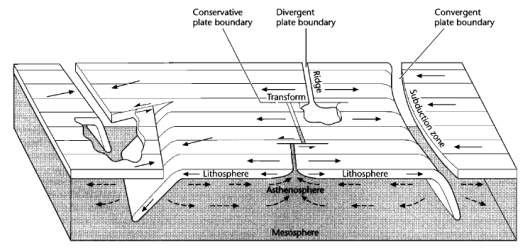
\includegraphics[width=6.86458in,height=\textheight]{./images/paste-4BA6D504.png} \hfill{}

\end{figure}

The mechanism in which governs the basin forming cannot be separated
from processes happening inside the lithosphere, which consist of
multiple plates interacting towards each others. This interaction
between plates is shown by the plate margins that moves towards each
other (convergent), separated toward each others (divergent), and plates
that are moving side-by-side each others (transform), as shown in
Figure~\ref{fig-basin-forming}.

According to {``Basin Analysis: Principles and Applications''} (2005),
basin-forming mechanism can be grouped into three categories:

\begin{enumerate}
\def\labelenumi{\arabic{enumi}.}
\item
  Isostatic consequences of changes in crustal/lithospheric thickness,
  caused by the lithospheric stretching or purely caused by thermal,
  happening simultaneously with the cooling of sea crust which moves
  away from MOR (Mid-Oceanic Ridge) area.
\item
  Loading and unloading lithosphere, due to flexural deflection/
  deformation which can also be followed by uplifting and subsidence,
  similar to forefront basin forming.
\item
  Dynamic topography. Viscous flow from mantle that causes non-permanent
  uplifting and subsidence.
\end{enumerate}

Based on the three above points, there are two parent groups of
basin-forming, which are:

\begin{itemize}
\item
  Basin formed by the lithospheric stretching, can be a rift-drift
  (divergent movement), and
\item
  Basin formed by the flexing (flexural) of earth crust or sea crust.
\end{itemize}

\hypertarget{basin-forming}{%
\section{Basin Forming}\label{basin-forming}}

A basin can be formed only when there is a divergent force on the
lithosphere. In this sub-chapter, we will be discussing about the
mechanism based on litospheric stretching and flexural.

\hypertarget{lithospheric-stretching}{%
\subsection{Lithospheric Stretching}\label{lithospheric-stretching}}

Lithospheric stretching is a divergent move on plate that happened
because of the pull force of a plate. This force can be caused by pure
pull forces like in between plate margins that moves away from each
other (divergent), on the adjacent plate margin (transform) due to
second order force that creates pull-apart basin, or on plate margin
where it moves closer to each other (convergent) as a release-force
after compression regime.

When a lithosphere expoed to lithospheric stretching, astenosphere
(bottom part) will flow as more aqueous part, while the crust (upper
part) is rigid (brittle) will be exposed to cracking. These two
processes happening in the lithosphere will form a crust thinning which
will be causing a basin-forming.

There are three models available to explain these mechanism of crust
movement above astenosphere when lithospheric stretching happened:
McKenzie, Wernicke, and Cantilever model.

\begin{figure}

\sidecaption{\label{fig-mckenzie}McKenzie model (pure shear). This model
visualizes a ductile moves of a crust that undergone thinning, while the
brittle crust at top undergone a cracking (faults and grabens). This
model is characterized by the symmetry of its faults. {``Basin Analysis:
Principles and Applications''} (2005)}

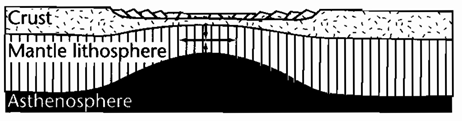
\includegraphics[width=6.78125in,height=\textheight]{./images/image-1782529132.png} \hfill{}

\end{figure}

\begin{figure}

\sidecaption{\label{fig-wernicke}Wernicke model (simple shear). This
model is characterized by the asymmetric movement between crust and
astenosphere {``Basin Analysis: Principles and Applications''} (2005)}

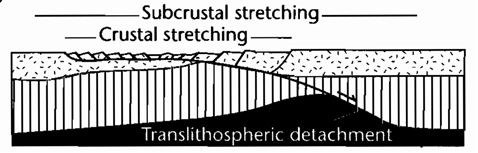
\includegraphics[width=6.83333in,height=\textheight]{./images/image-1735692408.png} \hfill{}

\end{figure}

\begin{figure}

\sidecaption{\label{fig-cantilever}Cantilever model (a combined model
between pure shear and simple shear). This model combines a simple shear
movement of the upper crust with pure shear movement of the mantle at
the bottom {``Basin Analysis: Principles and Applications''} (2005)}

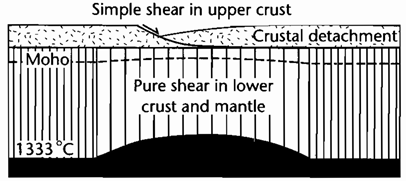
\includegraphics[width=6.72917in,height=\textheight]{./images/image-1564040352.png} \hfill{}

\end{figure}

\hypertarget{flexural-isostacy}{%
\subsection{Flexural Isostacy}\label{flexural-isostacy}}

Isostacy is a theory used to explain about the behavior of lithosphere
with astenosphere underneath. According to Airy, crust is distributed
according to similar density but different in the root length (column)
as depicted in the Figure~\ref{fig-airy} below.

\begin{figure}

\sidecaption{\label{fig-airy}Airy Isostacy model by Buchanan (1994)}

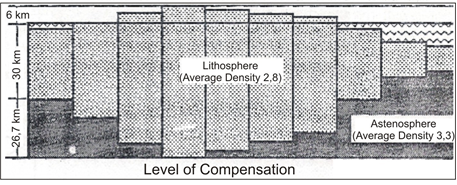
\includegraphics[width=6.69792in,height=\textheight]{./images/image-240741717.png} \hfill{}

\end{figure}

\bookmarksetup{startatroot}

\hypertarget{summary}{%
\chapter{Summary}\label{summary}}

In summary, this book has no content whatsoever.

\begin{Shaded}
\begin{Highlighting}[]
\DecValTok{1} \SpecialCharTok{+} \DecValTok{1}
\end{Highlighting}
\end{Shaded}

\begin{verbatim}
[1] 2
\end{verbatim}

\bookmarksetup{startatroot}

\hypertarget{references}{%
\chapter*{References}\label{references}}
\addcontentsline{toc}{chapter}{References}

\hypertarget{refs}{}
\begin{CSLReferences}{1}{0}
\leavevmode\vadjust pre{\hypertarget{ref-basinan2005}{}}%
{``Basin Analysis: Principles and Applications.''} 2005. \emph{Choice
Reviews Online} 43 (02). \url{https://doi.org/10.5860/choice.43-0957}.

\leavevmode\vadjust pre{\hypertarget{ref-buchanan1994}{}}%
Buchanan. 1994. \emph{Extensional Teconics and Basin Inversion}.

\leavevmode\vadjust pre{\hypertarget{ref-einsele2000}{}}%
Einsele, Gerhard. 2000. \emph{Sedimentary Basins}. Springer Berlin
Heidelberg. \url{https://doi.org/10.1007/978-3-662-04029-4}.

\end{CSLReferences}



\end{document}
